\documentclass{standalone}
\usepackage{graphicx}	
\usepackage{amssymb, amsmath, amsthm}
\usepackage{color}

\usepackage{tikz}
\usetikzlibrary{arrows.meta}

\definecolor{light}{RGB}{220, 188, 188}
\definecolor{mid}{RGB}{185, 124, 124}
\definecolor{dark}{RGB}{143, 39, 39}
\definecolor{highlight}{RGB}{180, 31, 180}
\definecolor{lightteal}{RGB}{107, 142, 142}
\definecolor{midteal}{RGB}{72, 117, 117}
\definecolor{darkteal}{RGB}{29, 79, 79}
\definecolor{gray10}{gray}{0.1}
\definecolor{gray20}{gray}{0.2}
\definecolor{gray30}{gray}{0.3}
\definecolor{gray40}{gray}{0.4}
\definecolor{gray60}{gray}{0.6}
\definecolor{gray70}{gray}{0.7}
\definecolor{gray80}{gray}{0.8}
\definecolor{gray90}{gray}{0.9}
\definecolor{gray95}{gray}{0.95}

\begin{document}

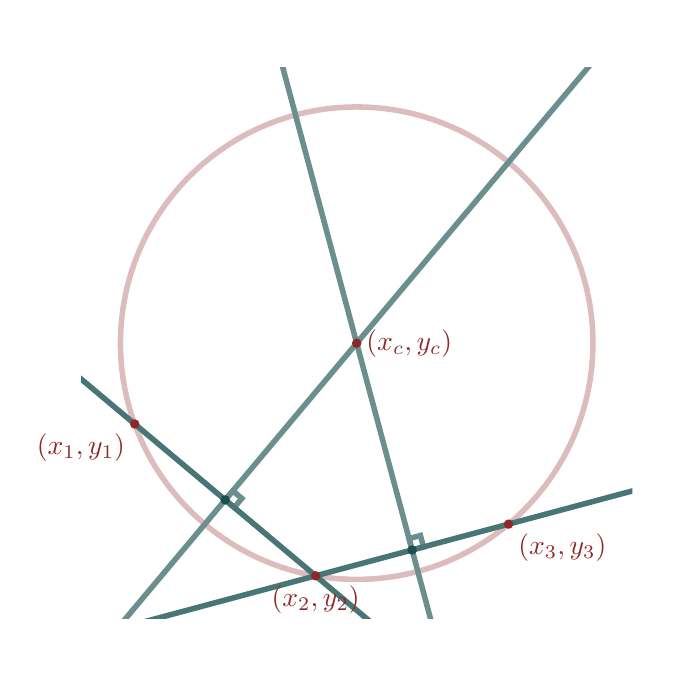
\begin{tikzpicture}

  \pgfmathsetmacro{\r}{3}

  \pgfmathsetmacro{\tha}{200}
  \pgfmathsetmacro{\xa}{\r * cos(\tha)}
  \pgfmathsetmacro{\ya}{\r * sin(\tha)}

  \pgfmathsetmacro{\thb}{260}
  \pgfmathsetmacro{\xb}{\r * cos(\thb)}
  \pgfmathsetmacro{\yb}{\r * sin(\thb)}
  
  \pgfmathsetmacro{\thc}{310}
  \pgfmathsetmacro{\xc}{\r * cos(\thc)}
  \pgfmathsetmacro{\yc}{\r * sin(\thc)}  
  
  \draw[white] (-4, -4) rectangle (4, 4);
  
  \draw[light, line width=2] (0, 0) circle (\r);

  \pgfmathsetmacro{\xab}{(\xa + \xb) / 2}
  \pgfmathsetmacro{\yab}{(\ya + \yb) / 2}
  
  \pgfmathsetmacro{\mab}{ ( \yb - \ya ) / ( \xb - \xa ) }
  \pgfmathsetmacro{\mabp}{-1 / \mab}
  
  \pgfmathsetmacro{\xbc}{(\xb + \xc) / 2}
  \pgfmathsetmacro{\ybc}{(\yb + \yc) / 2}

  \pgfmathsetmacro{\mbc}{ ( \yc - \yb ) / ( \xc - \xb ) }
  \pgfmathsetmacro{\mbcp}{-1 / \mbc}

  \begin{scope}
    \clip (-3.5, -3.5) rectangle (3.5, 3.5);
  
    \pgfmathsetmacro{\delta}{0.15}
    \draw[lightteal, line width=2, rotate around={atan(\mab):(\xab, \yab)}] 
      ( \xab, \yab ) rectangle +(\delta, \delta);
    \draw[lightteal, line width=2, rotate around={atan(\mbc):(\xbc, \ybc)}] 
      ( \xbc, \ybc ) rectangle +(\delta, \delta);
  
    \draw[lightteal, line width=2] 
      ( { (-4 - \yab ) / \mabp + \xab }, -4 ) -- ( 4, { \mabp * (4 - \xab ) + \yab });
    \draw[midteal, line width=2] 
      ( -4, { \mab * (-4 - \xa ) + \ya }) -- ( { (-4 - \ya ) / \mab + \xa }, -4 );
  
    \draw[lightteal, line width=2] 
      ( { (-4 - \ybc ) / \mbcp + \xbc }, -4 ) -- ( { (4 - \ybc ) / \mbcp + \xbc }, 4 ) ;
    \draw[midteal, line width=2] 
      ( { (-4 - \yb ) / \mbc + \xb }, -4 ) -- ( 4, { \mbc * (4 - \xb ) + \yb });
  \end{scope}
 
  \fill[dark] (0, 0) circle (0.06) node[right] { $(x_{c}, y_{c})$ };

  \fill[dark] (\xa, \ya) circle (0.06) node[below left] { $(x_{1}, y_{1})$ };
  \fill[dark] (\xb, \yb) circle (0.06) node[below] { $(x_{2}, y_{2})$ };
  \fill[dark] (\xc, \yc) circle (0.06) node[below right] { $(x_{3}, y_{3})$ };

  \fill[darkteal] (\xab, \yab) circle (0.06);
  \fill[darkteal] (\xbc, \ybc) circle (0.06); 

\end{tikzpicture}

\end{document}  